% =============================================================================
%  Romanization Flattens the Field  --  SHORT PAPER (4 pages of content)
%
%  COMPILER: XeLaTeX (required, for the Sinhala examples).
%  In Overleaf: Menu -> Compiler -> XeLaTeX.
%
%  This is the 4-page version. The 8-page version lives in ../paper/.
%  Switch \usepackage[review]{acl} to \usepackage{acl} for camera-ready.
% =============================================================================
\documentclass[11pt]{article}
\usepackage[review]{acl}

\usepackage{microtype}
\usepackage{graphicx}
\usepackage{booktabs}
\usepackage{amsmath}
\usepackage{amssymb}

% ---- fonts -------------------------------------------------------------------
\usepackage{fontspec}
\setmainfont{TeX Gyre Termes}
\setsansfont{TeX Gyre Heros}
\setmonofont{TeX Gyre Cursor}[Scale=MatchLowercase]

% Sinhala. If Overleaf cannot find this face, substitute "Noto Sans Sinhala".
\newfontfamily\sinhalafont{Noto Serif Sinhala}[Script=Sinhala, Scale=MatchLowercase]
\newcommand{\si}[1]{{\sinhalafont #1}}

% ---- helpers -----------------------------------------------------------------
\newcommand{\rom}[1]{\textit{#1}}
\newcommand{\bpb}{\textsc{bpb}}
\newcommand{\bpw}{\textsc{bpw}}
\newcommand{\bpc}{\textsc{bpc}}
\newcommand{\mcc}{\textsc{mcc}}
\newcommand{\pkg}{\texttt{sinlipi}}

% LaTeX's \input confuses the alignment scanner inside a tabular, so the
% machine-generated table bodies are pulled in with the TeX primitive instead.
\makeatletter
\newcommand{\rows}[1]{\@@input #1 }
\makeatother

% Float placement: the defaults leave too little room to keep two floats inside
% four pages.
\renewcommand{\topfraction}{0.92}
\renewcommand{\textfraction}{0.07}
\renewcommand{\floatpagefraction}{0.75}
\renewcommand{\dbltopfraction}{0.92}
\setcounter{topnumber}{3}
\setcounter{dbltopnumber}{3}

% Anonymous placeholders. Replace both before camera-ready.
\newcommand{\anonrepo}{\url{https://anonymous.4open.science/r/sinhala-script-robustness}}
\newcommand{\pkgurl}{\url{https://pypi.org/project/sinlipi}}

\title{Romanization Flattens the Field: Tokenizer-Independent and Downstream\\
Evidence of Script Fragility in Sinhala}

\author{Anonymous ACL submission}

\begin{document}
\maketitle

\begin{abstract}
Sinhala is written both in its native script and, in everyday digital use, romanized
in Latin letters. A recent benchmark reported that language models are some 300 times
worse on Romanized Sinhala and that model scale predicts nothing. We show both
conclusions are properties of the metric. Recomputing 31 checkpoints with
tokenizer-independent bits per byte, the perplexity and bits-per-byte rankings are
uncorrelated ($\rho = 0.08$) because perplexity mostly tracks how finely a tokenizer
shreds Sinhala, the 300-fold gap becomes 2.14 bits per byte, and scale does predict
native-script ability. We then run the first downstream evaluation of Sinhala script
variation, over three tasks, 9{,}479 items and ten instruction-tuned checkpoints in
both scripts. Romanization does not degrade models uniformly, it flattens them: the
loss is 0.78 times a checkpoint's above-chance headroom ($R^2 = 0.97$), a relation
holding again across 16 benchmark strata. Accuracy conceals this on offensive-language
detection, where Matthews correlation loses 60\% of its value.
\end{abstract}

% =============================================================================
\section{Introduction}
\label{sec:intro}

Sinhala has some 17 million speakers and a script of its own
\citep{ranasinghe-etal-2025-sold}. Like several South Asian languages it has an
everyday orthographic split: formal writing uses the native script, while chat and
social media are dominated by Romanized Sinhala, typed in Latin letters with no
standard spelling, so \si{කොහොමද} (``how are you'') appears as \rom{kohomada},
\rom{kohomd} or \rom{kohomade}. This is not marginal. For Indian languages,
\citet{khullar-etal-2025-scriptgap} found 83\% of Hindi and 73\% of Telugu messages
to a real health service were Romanized, and that models handled them worse. A
Sinhala system is therefore likely to serve mostly Romanized input while being
evaluated on native-script benchmarks.

\citet{rajapakse-weerasinghe-2026-script} gave the first systematic measurement,
benchmarking 24 open-weight models with perplexity and reporting a median 312-fold
degradation and no correlation between parameter count and script handling. Both rest
on a metric that is not comparable across models, since perplexity is normalised by
token count and token count depends entirely on the tokenizer
\citep{gao-etal-2020-pile, magnusson-etal-2024-paloma}, and Sinhala is where that
matters because tokenizers segment it very unevenly
\citep{petrov-etal-2023-tokenizers, ahia-etal-2023-languages}. That work also notes
perplexity says nothing about downstream ability, and calls for such evaluation. We
address both problems.

\paragraph{Related work.}
Sinhala is low-resource with fragmented tooling \citep{desilva-2019-survey,
ranathunga-de-silva-2022-languages, joshi-etal-2020-state} and its recent resources are
almost entirely native-script \citep{pramodya-etal-2025-sinhalammlu,
ranasinghe-etal-2025-sold, dhananjaya-etal-2022-bertifying, chang-etal-2025-globalpiqa}.
Romanized South Asian text has been studied mainly as a resource and identification
problem \citep{roark-etal-2020-dakshina, benton-etal-2025-improving}, and
\citet{j-etal-2024-romansetu} show romanization can \emph{help} when models are adapted
for it, the mirror image of our zero-shot setting. Tokenizers treat languages unequally
\citep{petrov-etal-2023-tokenizers, ahia-etal-2023-languages}, which is why bits per byte
exists \citep{gao-etal-2020-pile, magnusson-etal-2024-paloma}. To our knowledge ours is
the first work showing that, for a specific language, a published benchmark's conclusions
reverse when the normaliser changes.

\paragraph{C1: fixing the metric reverses the intrinsic conclusions.}
We recompute bits per byte, per character and per word for 31 checkpoints, 7 of them new,
on the same parallel corpus (\S\ref{sec:intrinsic}). Our perplexities reproduce the
published values, so what follows comes from the metric, not the measurement. Perplexity
and bits per byte are uncorrelated ($\rho = 0.08$, $p = 0.68$), while perplexity is almost
fully explained by tokenizer fertility ($\rho = -0.87$, $p < 10^{-9}$). The 300-fold gap is
2.14 bits per byte, and scale \emph{does} predict native-script ability
($\rho = -0.55$, $p = 0.001$), though still not Romanized ability.

\paragraph{C2: Romanization flattens, by a measurable law.}
We evaluate ten instruction-tuned checkpoints on 9{,}479 items across multiple-choice
knowledge, offensive-language detection and physical commonsense, in both scripts, for
189{,}580 generations (\S\ref{sec:extrinsic}). Native-script ability varies widely and
Romanized ability barely does: the loss is $0.78 \times$ a checkpoint's above-chance
headroom ($R^2 = 0.97$), and the same relation reappears across the 16 domain by
difficulty cells. The effect is neither a token-length artifact nor degeneration.

\paragraph{C3: what predicts fragility, and released artifacts.}
Absolute native-script bits per byte predicts the downstream gap
($\rho = -0.90$, $p = 0.0009$), whereas the bits-per-byte \emph{gap}, the quantity prior
work reports, predicts nothing ($\rho = -0.07$, $p = 0.86$). Building the Romanized side
needed a native-to-Latin transliterator, the opposite of the direction most Sinhala tools
support; ours beats three alternatives on 755{,}000 human references and is released with
the paired evaluation sets and all per-item generations
(Appendix~\ref{sec:artifacts}).

% =============================================================================
\section{Setup}
\label{sec:setup}

\paragraph{Conditions and data.}
Every item is scored twice, in the native script as published and romanized with
identical content, so all comparisons are paired and differ only in orthography. The
intrinsic corpus is the parallel set of \citet{rajapakse-weerasinghe-2026-script}: 500
sentence pairs whose Romanized side was \emph{typed by native speakers}, so those
results do not depend on our transliterator, plus 500 authentic mixed-script
sentences. Downstream we use every available item, with no sampling. SinhalaMMLU
\citep{pramodya-etal-2025-sinhalammlu} is 6{,}879 curriculum-aligned multiple-choice
items over six domains and three difficulty levels; 2{,}139 have five options, so
guessing scores 23.4\%, not 25\%.\footnote{The public release is an 1{,}851-item
sample. We obtained the full set from the authors.} SOLD
\citep{ranasinghe-etal-2025-sold} is the full 2{,}500-item offensive-language test
split, 40.6\% offensive, so the majority class scores 59.4\%. Global PIQA
\citep{desilva-ranathunga-2026-sinhalapiqa} adds 100 Sinhala items.

\paragraph{Transliteration.}
Almost all Sinhala tools run Latin to native \citep{de-mel-etal-2025-sinhala,
sumanathilaka-etal-2025-swabhasha}, so we wrote the reverse: a deterministic
grapheme-level transliterator using the conventions people type, \si{ත} as \rom{th} and
\si{ව} as \rom{w} not \rom{v}, so \si{වෙසක් උත්සවයේදී} becomes
\rom{wesak uthsawayeedii}. Against 755{,}000 human-romanized items
\citep{sumanathilaka-etal-2025-swabhasha} it has the lowest character error rate of four
methods on all three reference corpora, beating Aksharamukha
\citep{rajan-aksharamukha} and uroman \citep{hermjakob-etal-2018-uroman} at
$p < 10^{-90}$ (Appendix~\ref{sec:translit}).

\paragraph{Models and prompting.}
The intrinsic evaluation covers 31 decoder-only checkpoints from 350M to 14.7B across
eight families (Appendix~\ref{sec:models}). Downstream needs models that follow a
response format, so it uses the ten instruction-tuned checkpoints in the pool, 1.1B to
9B. All prompts are zero-shot and greedily decoded with a 40-token limit. One template,
chosen by a 3{,}240-generation pilot, is applied to every dataset and both conditions;
what matters for a paired comparison is not that the template be optimal but that it not
favour a script, and the pilot winner was the same under both scripts everywhere
(Appendix~\ref{sec:prompts}). Unparseable answers are scored wrong and reported as an
invalid rate.

\paragraph{Statistics and competence screen.}
Since both conditions score the same items we use McNemar's test
\citep{mcnemar-1947, dror-etal-2018-hitchhikers}, report discordant pair counts, and
control the family-wise error rate over checkpoints within each dataset with Holm's
procedure \citep{holm-1979}. Intervals come from 10{,}000 paired item bootstrap resamples.
For SOLD we lead with Matthews correlation \citep{matthews-1975, chicco-jurman-2020},
since the classes are imbalanced and accuracy sits near the majority baseline. A model at
chance natively cannot
lose anything by being given Romanized input, so a small gap for it is evidence of
nothing and averaging it in understates the effect. We therefore mark a checkpoint
\emph{competent} on a task when its native score beats the guessing baseline at
$p < 0.01$ under a Poisson-binomial null and it puts at most 90\% of answers on one
option. Five of ten pass on SinhalaMMLU, five have a non-trivial SOLD signal, none
pass on Global PIQA, and all ten appear in every table.

% =============================================================================
\section{Perplexity Measures Tokenizers}
\label{sec:intrinsic}

We divide the total negative log-likelihood in nats by a unit of the text itself
rather than by its tokenization,
$\bpb = \sum_s \mathrm{NLL}(s) \,/\, (\ln 2 \sum_s |s|_{\text{bytes}})$, and likewise
per character (\bpc) and per whitespace word (\bpw), pooling numerator and denominator
over the corpus so short sentences do not dominate. Bytes are standard
\citep{gao-etal-2020-pile}, but \bpw{} is sharpest across scripts, since a sentence and its
romanization contain the same number of words while Sinhala UTF-8 spends 2.65 bytes per
character against 1.00 for Latin. Our perplexities reproduce the published values for all
24 shared checkpoints, median absolute deviation 0.05\% native and 0.004\% Romanized.

\paragraph{The two metrics disagree.}
Figure~\ref{fig:metric}(a) is the methodological result. Native-script perplexity and
bits per byte are statistically unrelated ($\rho = 0.08$, $p = 0.68$; Romanized
$\rho = 0.13$, $p = 0.48$), only one of the five best checkpoints by perplexity is among
the five best by bits per byte, and Gemma-2-9B ranks 26th of 31 on perplexity but 2nd on
bits per byte. The cause is the colour axis: perplexity is almost fully explained by
tokens spent per Sinhala word ($\rho = -0.87$, $p < 10^{-9}$), from 4.3 for the Qwen3.5
and Gemma tokenizers to 14.2 for models falling back to bytes. Spreading the same loss
over three times as many tokens lowers per-token perplexity without the model knowing
more, so a cross-family perplexity comparison here is largely a comparison of
tokenizers.

Two published conclusions do not survive. The 312-fold degradation is mostly
tokenization: our median ratio is 294-fold, but the same gap is 2.14 bits per byte and
1.11 bits per word. And scale is uncorrelated with native perplexity
($\rho = 0.15$, $p = 0.42$) yet correlated with native bits per byte
($\rho = -0.55$, $p = 0.001$). Scale does buy native-script ability; what it does not buy
is Romanized ability ($\rho = -0.28$, $p = 0.13$).

\paragraph{Flattening, and an absolute reference.}
Native-script cost spans 16.3 to 34.1 bits per word across checkpoints while Romanized
cost spans only 20.3 to 25.7, so a full bit per word of native improvement buys 0.14
bits on Romanized text (95\% CI $[0.05, 0.25]$), and 12 of 31 checkpoints are actually
\emph{cheaper} on Romanized than on native Sinhala: the better a checkpoint is
natively, the more it loses ($\rho = -0.88$, Appendix~\ref{sec:flat}). Mixed script instead
reproduces the earlier finding, rank-correlated with native at $\rho = 0.94$, so
interleaving scripts is a mild perturbation where replacing one is not. To calibrate
absolutely, add-$\alpha$ character $n$-gram models fit on the same corpus under five-fold
cross-validation reach 2.64 bits per byte on Romanized Sinhala and a character bigram
reaches 3.06, while the best of 31 checkpoints reaches 3.29 and the median 3.81: not one
beats the bigram, though on native Sinhala the trigram is at 1.16 with one checkpoint
below it (Appendix~\ref{sec:ngram}). Whatever these checkpoints know about Sinhala, they
know it about the script rather than the language.

\begin{table*}[t]
\centering\footnotesize
\setlength{\tabcolsep}{2.4pt}
\begin{tabular}{@{}lr rrr c@{\hspace{3pt}}r rr rr r rr r@{}}
\toprule
& & \multicolumn{5}{c}{\textbf{SinhalaMMLU} (6{,}879 items)}
& \multicolumn{5}{c}{\textbf{SOLD} (2{,}500 items)}
& \multicolumn{2}{c}{\textbf{Invalid \%}} & \\
\cmidrule(lr){3-7}\cmidrule(lr){8-12}\cmidrule(lr){13-14}
& & \multicolumn{2}{c}{Acc.\ \%} & & &
& \multicolumn{2}{c}{macro-F1} & \multicolumn{2}{c}{\mcc} & & & & \\
\textbf{Checkpoint} & \textbf{B} & U & R & $\Delta$ & 95\% CI & $p_{\text{Holm}}$
& U & R & U & R & $p_{\text{Holm}}$ & U & R & $\tau$ \\
\midrule
\rows{tables/tab_extrinsic_main.tex}
\bottomrule
\end{tabular}
\caption{Downstream results by size. U is native Unicode, R Romanized, $\Delta$ the
paired difference in points, $p_{\text{Holm}}$ McNemar's test corrected across
checkpoints within a task ($\mcc$: paired bootstrap). $\tau$ is Romanized over native
input tokens on SinhalaMMLU, below one throughout. Invalid \% is unparseable
generations. $\dagger$ passes the competence screen (\S\ref{sec:setup}).}
\label{tab:main}
\end{table*}

\begin{figure}[t]
\centering
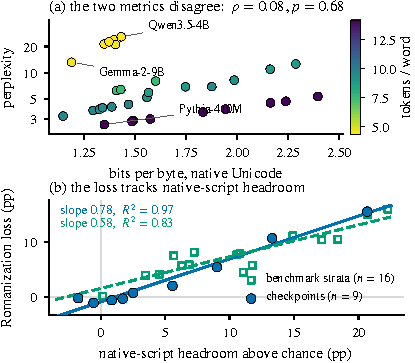
\includegraphics[width=\columnwidth]{figures/figS1_metric_and_law.pdf}
\caption{(a) Native-script perplexity is unrelated to native-script bits per byte
across 31 checkpoints, and is instead determined by tokenizer fertility (colour).
(b) Romanization loss against native-script headroom above chance, measured
independently across checkpoints and across the 16 domain by difficulty cells of
SinhalaMMLU.}
\label{fig:metric}
\end{figure}

% =============================================================================
\section{Downstream Consequences}
\label{sec:extrinsic}

\paragraph{Multiple-choice knowledge.}
Table~\ref{tab:main} reports every checkpoint. Four of the five competent checkpoints lose
significantly after Holm correction: Qwen3.5-9B falls from 44.1\% to 28.7\%, a 15.5 point
drop (95\% CI $[14.0, 16.9]$, 1{,}892 against 828 discordant pairs), Qwen3.5-4B loses
10.6, Llama-3.1-8B-Instruct 5.4 and Qwen2-7B-Instruct 2.0. The fifth, Hormoz-8B, starts
only 2.5 points above chance and loses 0.8, not significant. Pooled the gap is 6.9 points
(95\% CI $[6.3, 7.5]$, $n = 34{,}395$ paired items), and a logistic fit with checkpoint
fixed effects and item-clustered errors puts the odds ratio for Romanized input at 0.68
($p < 10^{-30}$). Read as levels this is starker: native accuracy spans 22.4 points and
Romanized only 6.7, never exceeding 28.7\% against a 23.4\% baseline, so the best
checkpoint keeps 5.2 of its 20.7 points of headroom, and the six checkpoints showing no
gap are the six already at chance.

\paragraph{You can only lose what you have.}
That relation is tight. Writing headroom as native accuracy minus chance, a fit across
the nine parseable checkpoints gives
\begin{equation}
\text{loss} = 0.78 \times \text{headroom} - 0.87,
\label{eq:law}
\end{equation}
with $R^2 = 0.97$ and $p = 1.9 \times 10^{-6}$ (Figure~\ref{fig:metric}b): Romanization
removes roughly four fifths of whatever native ability a checkpoint had. A regression on
nine points is thin, so we test the same relation inside the benchmark, where the units are
items rather than models: over the 16 non-empty domain by difficulty cells, headroom and
loss per cell give a slope of 0.58 with $R^2 = 0.83$ ($p = 9.8 \times 10^{-7}$). The two decompositions are independent, one across models and one
across content, and they agree. Loss also falls monotonically with difficulty, 8.6 points
on Easy to 5.2 on Hard ($p = 0.007$ for the interaction), because Hard items sit nearer
chance in both conditions (Appendix~\ref{sec:strata}): the harder a slice, the smaller the
script effect it can reveal.

\paragraph{Accuracy hides the damage on SOLD.}
Accuracy falls by only 1.6 to 11.3 points against a 59.4\% majority baseline, so three
checkpoints look almost unaffected. Matthews correlation says otherwise: Qwen3.5-9B goes
from 0.280 to 0.069, keeping 24\% of its signal, Qwen2-7B-Instruct from 0.148 to 0.042
(29\%) and Llama-3.1-8B-Instruct from 0.259 to 0.105 (40\%). Four of the five checkpoints
with a real native signal lose significantly under Holm correction and the median keeps
40\%. The mechanism is a retreat toward trivial behaviour: Qwen2-7B-Instruct more than
doubles its rate of predicting the offensive class, 10.5\% to 23.4\%, without becoming
more accurate. A deployment tracking accuracy would see a 5 point wobble while over half
the usable signal disappeared.

\paragraph{Two things it is not.}
The natural explanation is that romanization shatters words into more tokens. For Sinhala
the opposite holds: the native script costs a median 9.5 tokens per word against 2.09 for
its romanization, because these tokenizers largely fall back to bytes, and all ten
checkpoints receive \emph{fewer} tokens in the Romanized condition on all three tasks, a
median ratio of 0.48 (column $\tau$). Models get shorter, more compactly encoded input and
do worse, and terciles by token inflation show no monotone pattern either. Nor is this
degeneration: the most frequent option takes 37.0\% of answers natively and 38.6\%
romanized (Wilcoxon $p = 0.63$) and the invalid rate never exceeds 0.03\% for competent
checkpoints, so models keep answering and are simply wrong. Global PIQA is a null result
(Appendix~\ref{sec:piqa}).

\paragraph{What this means in practice.}
Perplexity reported across model families on a script tokenizers handle unevenly measures
tokenizer behaviour, which for Sinhala inverts both the ranking and the conclusion about
scale. Script robustness also cannot be read off a group average, since six of our ten
checkpoints contribute a zero gap by construction, so such claims need a competence screen
and a stated baseline.


% =============================================================================
\section*{Limitations}

\paragraph{One language.} Everything here is Sinhala. The mechanism, a floor effect
making robustness gaps proportional to native ability, should generalise to any
language with a dominant Romanized register, but we have not shown that. Hindi, Urdu,
Nepali, Tamil and Arabic dialects are the obvious tests, and
\citet{khullar-etal-2025-scriptgap} report compatible magnitudes for the first three.

\paragraph{The Romanized downstream side is synthetic.} We transliterate
native-script items rather than collecting human-typed Romanized versions, because no
parallel resource exists at this scale. Our transliterator is the best of four on
755{,}000 human references, and its residual error is a spelling regularity that
should make the text easier rather than harder, but it is not what a person would
type. The intrinsic results do not share this limitation, since their Romanized side
was typed by native speakers, and they show the same flattening. A human-written
Romanized version of even a few hundred SinhalaMMLU items would settle the question.

\paragraph{Open weights only, and small ones.} The downstream evaluation covers open
checkpoints up to 9B. Frontier proprietary models are much stronger on Sinhala
\citep{pramodya-etal-2025-sinhalammlu} and so have far more headroom, which means
Equation~\ref{eq:law} predicts larger absolute losses for them. That prediction is
untested here.

\paragraph{Zero-shot only.} One template, zero-shot, greedy. This measures what a
user gets out of the box, not the ceiling. Few-shot prompting,
transliterate-then-infer, or Romanized fine-tuning could all narrow the gap and we do
not measure by how much.

\paragraph{Two checkpoints cannot do the task.} LaMini-GPT-1.5B and
TinyLlama-1.1B-Chat produce unparseable output on most native-script items of at least
one task, so their apparent improvement under Romanization is an artifact of that
failure rather than a script effect. This is why the competence screen exists.

\paragraph{The $n$-gram comparison is not matched.} The $n$-gram models are fit
in-domain on held-out folds of the same corpus while the checkpoints are zero-shot.
The comparison establishes an absolute floor, not a like-for-like ranking.

\section*{Ethics Statement}

All datasets are public research releases used within their licences and for
evaluation only, which matters for Global PIQA, whose licence forbids training. SOLD
contains offensive social media text, already pseudonymised upstream with user
mentions replaced by placeholders; we neither collected nor re-annotated any of it,
and we add no new human annotation. The practical risk our results speak to is
deployment: a moderation or support system validated on native-script Sinhala and
serving Romanized users will look far better in evaluation than in the field, and on
SOLD that failure is invisible in accuracy while more than half the usable signal is
gone. Our transliterator collapses several Sinhala consonant distinctions, matching
casual practice, so it is a tool for building evaluation data rather than for
rendering names or other text where those distinctions carry meaning.

\section*{Acknowledgments}

Omitted for anonymous review.

\bibliography{custom}

% =============================================================================
\appendix

\section{Released Artifacts and Reproducibility}
\label{sec:artifacts}

We release three artifacts at \anonrepo. The \textbf{transliterator}
(\texttt{pip install \pkg}, \pkgurl) is local, deterministic, covers every input and is
the best of four methods on 755{,}000 human references, which makes Romanized
evaluation data cheap to build for any native-script Sinhala resource. The
\textbf{frozen evaluation sets} pair both script conditions in one record per item,
regenerable byte-identically with SHA-256 digests recorded, so a paired analysis cannot
compare mismatched subsets. The \textbf{harness and analysis pipeline} ships all
189{,}580 per-item generations, the statistics, the figure and table generators, and a
checker that restates every number in this paper and verifies it against the analysis
output, so the reported values cannot drift from the data.

\section{Prompt Template and Compute}
\label{sec:prompts}

SinhalaMMLU follows MMLU \citep{hendrycks-etal-2021-mmlu} and Global PIQA follows PIQA
\citep{bisk-etal-2020-piqa}. One template is used for every dataset and both script
conditions. Multiple choice, with the option count $n$ and the domain name inserted where
available:

\begin{quote}\small\ttfamily
This is a multiple-choice question related to the \{domain\}. Choose the correct or
most appropriate answer from answers 1/.../$n$ for the following question. Do not
repeat the question or text in your response. Respond with only the number
(1/.../$n$) and nothing else.\\
Question: \{question\}\\
1. \{option 1\} ... $n$. \{option $n$\}\\
Answer:
\end{quote}

Binary classification:

\begin{quote}\small\ttfamily
Classify the following Sinhala text as either 'NOT' (not offensive) or 'OFF'
(offensive). Do not repeat the question or text in your response. Respond with only
'NOT' or 'OFF' and nothing else.\\
Text: \{text\}\\
Answer:
\end{quote}

Prompts are rendered through each checkpoint's own chat template. For checkpoints that
emit reasoning traces by default we disable that behaviour identically in both script
conditions. Decoding is greedy at temperature 0 with at most 40 new tokens and inputs
truncated at 4{,}096 tokens. Models run in fp16 on dual T4 GPUs. Intrinsic evaluation
scores 46{,}500 sequences (31 checkpoints, 1{,}500 each); downstream evaluation
produces 189{,}580 generations (10 checkpoints, 9{,}479 items, two conditions).

\section{Flattening}
\label{sec:flat}

\begin{figure}[h]
\centering
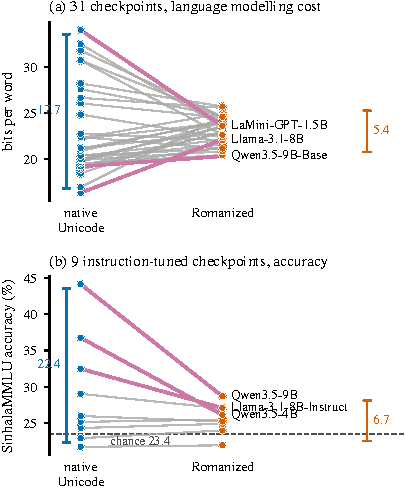
\includegraphics[width=\columnwidth]{figures/figS2_flattening_narrow.pdf}
\caption{Romanization flattens the field. (a) Language modelling cost in bits per word
for 31 checkpoints; word counts are identical within a pair, so the two columns are
directly comparable. Native-script cost varies by 17.7 bits across checkpoints,
Romanized cost by 5.4, and crossing lines mark the twelve checkpoints cheaper on
Romanized text. (b) SinhalaMMLU accuracy. A 22.4 point spread becomes 6.7, and no
checkpoint finishes more than 5.3 points above chance. Brackets give each column's
spread. LaMini-GPT-1.5B is omitted from (b) because it produces unparseable output on
95.9\% of native-script items; it appears in Table~\ref{tab:main}.}
\label{fig:flat}
\end{figure}

\section{Character $n$-gram Reference}
\label{sec:ngram}

\begin{table}[h]
\centering\small
\setlength{\tabcolsep}{4pt}
\begin{tabular}{@{}lcccc@{}}
\toprule
& \multicolumn{2}{c}{\textbf{Native Unicode}} & \multicolumn{2}{c}{\textbf{Romanized}} \\
\cmidrule(lr){2-3}\cmidrule(lr){4-5}
\textbf{Model} & \bpb{} & \#\,LMs $<$ & \bpb{} & \#\,LMs $<$ \\
\midrule
\rows{tables/tab_ngram.tex}
\bottomrule
\end{tabular}
\caption{Held-out character $n$-gram models against the 31 checkpoints.
``\#\,LMs $<$'' counts checkpoints reaching lower bits per byte than the $n$-gram
model. No checkpoint beats a character bigram on Romanized Sinhala.}
\label{tab:ngram}
\end{table}

\section{Transliteration Evaluation}
\label{sec:translit}

Each hypothesis is scored against the closest accepted human variant, case-folded, using
character error rate, chrF \citep{popovic-2015-chrf} and exact match.
Case is folded because the web tool capitalises the first letter of whatever it is
given, an interface artifact rather than a romanization choice, and scoring
case-sensitively would reward it for that alone. The web tool is close once its
\rom{v} is rewritten to \rom{w}, a spelling convention rather than a transliteration
error, but it cannot romanize 17 sequences involving \si{ඤ} at all and leaves Sinhala
characters in 0.8\% to 2.5\% of its output. All four methods double long vowels far
more often than people do, 0.81 per word against 0.12, which is the dominant residual
error; canonicalising that single convention on both sides cuts our character error
rate to 0.040 on the word corpus.

\begin{table}[h]
\centering\small
\setlength{\tabcolsep}{2.2pt}
\begin{tabular}{@{}lccccc c@{}}
\toprule
& \multicolumn{3}{c}{\textbf{CER} $\downarrow$} & \textbf{chrF} & \textbf{Exact} & \textbf{Cov.} \\
\cmidrule(lr){2-4}\cmidrule(lr){5-5}\cmidrule(lr){6-6}\cmidrule(lr){7-7}
\textbf{Method} & sent. & word & aug. & sent. & word & \% \\
\midrule
\rows{tables/tab_methods.tex}
\bottomrule
\end{tabular}
\caption{Transliteration quality against human references: 4{,}397 authentic
social-media sentence pairs, 450{,}587 multi-reference words, and a fixed
300{,}000-sentence sample of a machine-augmented set used only as a cross-check.
Coverage is the share of inputs the method produced any output for.}
\label{tab:methods}
\end{table}

\section{SinhalaMMLU Strata}
\label{sec:strata}

\begin{table}[h]
\centering\small
\setlength{\tabcolsep}{4pt}
\begin{tabular}{@{}lrrrrr@{}}
\toprule
\textbf{Stratum} & \textbf{Items} & \textbf{U \%} & \textbf{R \%}
& \boldmath$\Delta$ & \boldmath$p_{\text{Holm}}$ \\
\midrule
\rows{tables/tab_strata.tex}
\bottomrule
\end{tabular}
\caption{SinhalaMMLU by stratum, pooled over the five competent checkpoints. Item
counts are per checkpoint. Domains are ordered by loss.}
\label{tab:strata}
\end{table}

\section{Intrinsic to Downstream Linkage}
\label{sec:linkage}

\begin{table}[h]
\centering\small
\setlength{\tabcolsep}{4pt}
\begin{tabular}{@{}lrrrr@{}}
\toprule
& \multicolumn{2}{c}{\textbf{MMLU gap}} & \multicolumn{2}{c}{\textbf{SOLD} $\Delta\mcc$} \\
\cmidrule(lr){2-3}\cmidrule(lr){4-5}
\textbf{Intrinsic predictor} & $\rho$ & $p$ & $\rho$ & $p$ \\
\midrule
\rows{tables/tab_linkage.tex}
\bottomrule
\end{tabular}
\caption{Spearman correlations between intrinsic measurements and downstream script
effects over the nine parseable checkpoints. Levels predict; gaps and ratios do not.}
\label{tab:linkage}
\end{table}

\section{Global PIQA}
\label{sec:piqa}

\begin{table}[h]
\centering\footnotesize
\setlength{\tabcolsep}{2.2pt}
\begin{tabular}{@{}lrrrcrrr@{}}
\toprule
& \multicolumn{2}{c}{Acc.\ \%} & & \textbf{disc.} & & \multicolumn{2}{c}{\textbf{Inv.\ \%}} \\
\cmidrule(lr){2-3}\cmidrule(lr){5-5}\cmidrule(lr){7-8}
\textbf{Checkpoint} & U & R & \boldmath$\Delta$ & \textbf{b/c}
& \boldmath$p_{\text{Holm}}$ & U & R \\
\midrule
\rows{tables/tab_piqa.tex}
\bottomrule
\end{tabular}
\caption{Global PIQA, 100 items. ``disc.\ b/c'' are the discordant pair counts
entering McNemar's test.}
\label{tab:piqa}
\end{table}

\section{Checkpoints and Full Intrinsic Results}
\label{sec:models}

\begin{table*}[h]
\centering\scriptsize
\setlength{\tabcolsep}{3pt}
\begin{tabular}{@{}lr rrr rrr rrr l@{}}
\toprule
& & \multicolumn{3}{c}{\textbf{Native Unicode}} & \multicolumn{3}{c}{\textbf{Romanized}}
& \multicolumn{3}{c}{\textbf{Mixed script}} & \\
\cmidrule(lr){3-5}\cmidrule(lr){6-8}\cmidrule(lr){9-11}
\textbf{Checkpoint} & \textbf{B} & PPL & \bpb{} & \bpw{}
& PPL & \bpb{} & \bpw{} & PPL & \bpb{} & \bpw{} & \textbf{Hugging Face identifier} \\
\midrule
\rows{tables/tab_intrinsic_joined.tex}
\bottomrule
\end{tabular}
\caption{Corpus-pooled intrinsic metrics for all 31 checkpoints, sorted by native-script
bits per byte, with Hugging Face identifiers. The pool spans the Llama
\citep{grattafiori-etal-2024-llama3}, Qwen \citep{yang-etal-2024-qwen2,
yang-etal-2025-qwen3}, Gemma \citep{gemmateam-2024-gemma2}, Mistral, BLOOM
\citep{lescao-etal-2023-bloom, laurencon-etal-2023-roots}, OPT, Pythia
\citep{biderman-etal-2023-pythia} and Phi \citep{abdin-etal-2024-phi4} families. $\ddagger$ marks the ten
evaluated downstream. Bits per character are omitted because within a script they are
a fixed multiple of bits per byte, $2.651\times$ for native Sinhala and
$1.003\times$ for its romanization. Note that the PPL and \bpb{} orderings disagree
almost completely.}
\label{tab:intrinsicfull}
\end{table*}

\end{document}
